%%%%%%%%%%%%%%%%%%%%%%%%%%%%%%%%%%%%
%% PREAMBLE
%%%%%%%%%%%%%%%%%%%%%%%%%%%%%%%%%%%%

\documentclass[11pt]{article}

% packages needed for state diagrams
\usepackage{pgf}
\usepackage{tikz}
\usetikzlibrary{arrows,automata}

% package needed for parse trees
\usepackage{qtree}

% nice clickable URLs
\usepackage{url}

% page margins
\usepackage[margin=2.5cm]{geometry}
\setlength{\parindent}{0pt}

\begin{document}

%%%%%%%%%%%%%%%%%%%%%%%%%%%%%%%%%%%%
%% HEADING
%%%%%%%%%%%%%%%%%%%%%%%%%%%%%%%%%%%%
\rule{\textwidth}{1pt}

\textbf{Taaltheorie en Taalverwerking}

\rule{\textwidth}{1pt}

\begin{center}\bf
\LaTeX\ resources for homework assignments
\end{center}
\vspace*{10pt}

%%%%%%%%%%%%%%%%%%%%%%%%%%%%%%%%%%%%
%% BODY
%%%%%%%%%%%%%%%%%%%%%%%%%%%%%%%%%%%%

% Regex
% ===========

\paragraph{Regular expressions in math notation:} To write regular expressions using
the notation introduced in class, use math mode. For instance:

$\Sigma =\{0,1\}$

$00(1)^+(100)^*$

$(010^*1)^*1(0|1)$

\paragraph{Regular expressions in Perl/Python notation:}
To write regular expressions in Perl/Python notation, use the \texttt{verbatim} environment. For instance:

\begin{verbatim}
baaa*!
gupp(y|ies)
^The dog\.$
[^a-aA-Z][tT]he[^a-zA-Z]
\end{verbatim}


% FSAs
% ===========

\paragraph{Finite state diagrams:}
To create finite state automata, use the \texttt{tikzpicture} environment.
Here are a few examples:

% FSA
% ===================

\begin{center}
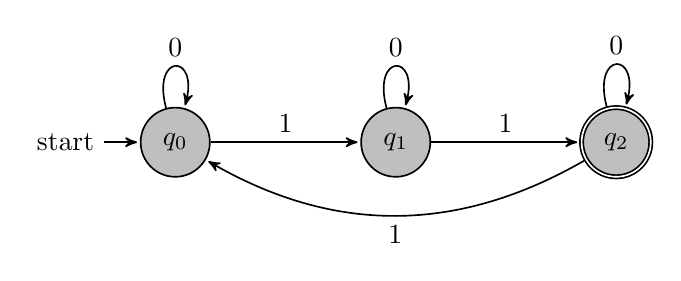
\begin{tikzpicture}[->,>=stealth',shorten >=1pt,auto,node distance=2.8cm,semithick]
  \tikzstyle{every state}=[fill=lightgray,draw=black,text=black]
\node[initial,state] (q0) {$q_0$};
\node[state] (q1) [right of=q0] {$q_1$};
\node[state,accepting] (q2) [right of=q1] {$q_2$};
\path
(q0) edge node {1} (q1) edge [loop above] node {0} (q1)
(q1) edge node {1} (q2) edge [loop above] node {0} (q2)
(q2) edge [loop above] node {0} (q2)
(q2) edge [bend left] node {1} (q0);
\end{tikzpicture}
\end{center}


% NFSA
% =====================

\begin{center}
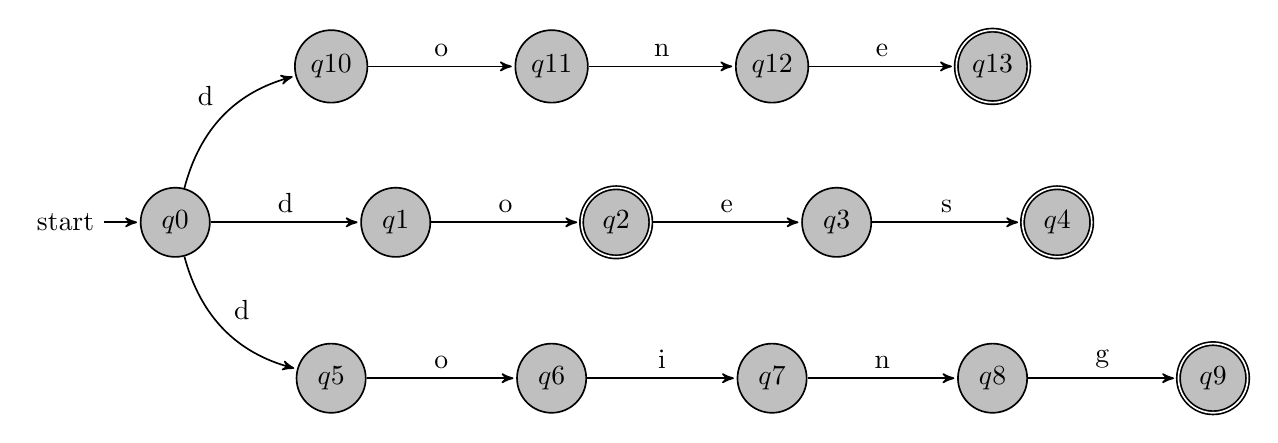
\begin{tikzpicture}[->,>=stealth',shorten >=1pt,auto,node distance=2.8cm,semithick]
  \tikzstyle{every state}=[fill=lightgray,draw=black,text=black]
\node[initial,state] (q0) {$q0$};
\node[state] (q1) [right of=q0] {$q1$};
\node[state,accepting] (q2) [right of=q1] {$q2$};
\node[state] (q3) [right of=q2] {$q3$};
\node[state,accepting] (q4) [right of=q3]{$q4$};
\node[state] (q5) [below right of=q0] {$q5$};
\node[state] (q6) [right of=q5] {$q6$};
\node[state] (q7) [right of=q6] {$q7$};
\node[state] (q8) [right of=q7] {$q8$};
\node[state,accepting] (q9) [right of=q8] {$q9$};
\node[state] (q10) [above right of=q0] {$q10$};
\node[state] (q11) [right of=q10] {$q11$};
\node[state] (q12) [right of=q11] {$q12$};
\node[state,accepting] (q13) [right of=q12] {$q13$};
\path
(q0) edge node {d} (q1)
(q1) edge node {o} (q2)
(q2) edge node {e} (q3)
(q3) edge node {s} (q4)
(q0) edge [bend left] node {d} (q10)
(q10) edge node {o} (q11)
(q11) edge node {n} (q12)
(q12) edge node {e} (q13)
(q0) edge [bend right] node {d} (q5)
(q5) edge node {o} (q6)
(q6) edge node {i} (q7)
(q7) edge node {n} (q8)
(q8) edge node {g} (q9);
\end{tikzpicture}
\end{center}

% FST
% =====================

\begin{center}
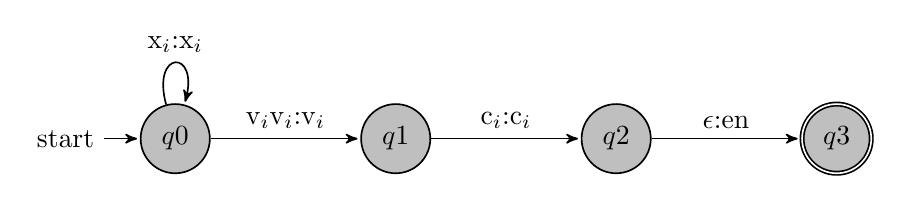
\begin{tikzpicture}[->,>=stealth',shorten >=1pt,auto,node distance=2.8cm,semithick]
  \tikzstyle{every state}=[fill=lightgray,draw=black,text=black]

\node[initial,state] (0) {$q0$};
\node[state] (1) [right of=0] {$q1$};
\node[state] (2) [right of=1] {$q2$};
\node[state,accepting] (3) [right of=2] {$q3$};

\path
(0) edge [loop above] node {x$_i$:x$_i$} (0)
(0) edge node {v$_i$v$_i$:v$_i$} (1)
(1) edge node {c$_i$:c$_i$} (2)
(2) edge node {$\epsilon$:en} (3);
\end{tikzpicture}
\end{center}


% Trees
% ===========

\paragraph{Syntactic trees.} A few examples:


\paragraph{Example 1:}

\Tree [.A [.B [.C one ] [.D two ] ].B [.E three ] ].A


\paragraph{Example 2:}

\Tree [.S This [.VP [.V is ] \qroof{a simple tree}.NP ] ]


\paragraph{Example 3:}

\Tree[.S [.NP [.Det the ] [.N tourist ]]
[.VP [.V saw ] [.NP [.NP [.Det the ] [.N astronomer ]]
[.PP [.P with ] [.NP [.Det the ] [.N telescope ]]]]]]


%%%%%%%%%%%%%%%%%%%%%%%%%%%%%%%%%%%%
%% END
%%%%%%%%%%%%%%%%%%%%%%%%%%%%%%%%%%%%

\end{document}
